\documentclass[brazil, english]{ufsc-thesis}

\usepackage[T1]{fontenc} % fontes
\usepackage[utf8]{inputenc} % UTF-8
\usepackage{lipsum} % Gerador de texto
\usepackage{pdfpages} % Inclui PDF externo (ficha catalográfica)
\usepackage{tikz} % tikz
\usepackage{amsfonts}
\usepackage{amsmath}
\usepackage[ruled,linesnumbered]{algorithm2e} % algorithms
\usepackage{tabularx} % protocol
\usepackage{url}


%%%%%%%%%%%%%%%%%%%%%%%%%%%%%%%%%%%%%%%%%%%%%%%%%%%%%%%%%%%%%%%%%%%%
%%% Configurações da classe (dados do trabalho)                  %%%
%%%%%%%%%%%%%%%%%%%%%%%%%%%%%%%%%%%%%%%%%%%%%%%%%%%%%%%%%%%%%%%%%%%%
\titulo{Root finding techniques in binary finite fields}
\autor{Douglas Marcelino Beppler Martins}
\data{1 de Agosto de 2019}
\instituicao{Universidade Federal de Santa Catarina}
\centro{Centro Tecnológico}
\programa{Programa de Pós-Graduação em Ciência da Computação}
\dissertacao
\local{Florianópolis}
\titulode{Mestre em Ciência da Computação}

%%%%%%%%%%%%%%%%%%%%%%%%%%%%%%%%%%%%%%%%%%%%%%%%%%%%%%%%%%%%%%%%%%%%
%%% Membros da banca (Dr. depois)                                %%%
%%%%%%%%%%%%%%%%%%%%%%%%%%%%%%%%%%%%%%%%%%%%%%%%%%%%%%%%%%%%%%%%%%%%
\orientador{Prof. Ricardo Felipe Custódio, Dr.}
\membrobanca{Prof. Daniel Panario, Dr.}
{Carleton University}
\membrobanca{Prof. Jean Everson Martina, Dr.}
{Universidade Federal de Santa Catarina}
\membrobanca{Prof. Huifen Chan, Dr.}
{Universidade Federal de Santa Catarina}
\coordenadora{Prof. Vania Bogorny, Dr}

\DeclareMathAlphabet{\mathcal}{OMS}{cmsy}{m}{n}


%%%%%%%%%%%%%%%%%%%%%%%%%%%%%%%%%%%%%%%%%%%%%%%%%%%%%%%%%%%%%%%%%%%%
%%% Protocol environment                                         %%%
%%%%%%%%%%%%%%%%%%%%%%%%%%%%%%%%%%%%%%%%%%%%%%%%%%%%%%%%%%%%%%%%%%%%
\newcounter{protocol}
\newenvironment{protocol}[1]
  {\noindent
   \tabularx{\linewidth}{@{} X @{}}
    \hline
    \vspace{-3mm}
    \refstepcounter{protocol}\hspace{7.5mm}\textbf{Protocol \theprotocol:} #1 \\
    \hline}
    {\endtabularx}

\newcommand{\sbline}{\\[.5\normalbaselineskip]}% small blank line

\begin{document}
%%%%%%%%%%%%%%%%%%%%%%%%%%%%%%%%%%%%%%%%%%%%%%%%%%%%%%%%%%%%%%%%%%%%
%%% Principais elementos pré-textuais                            %%%
%%%%%%%%%%%%%%%%%%%%%%%%%%%%%%%%%%%%%%%%%%%%%%%%%%%%%%%%%%%%%%%%%%%%

% Inicia parte pré-textual do documento capa, folha de rosto, folha de
% aprovação, aprovação, resumo, lista de tabelas, lista de figuras, etc.
\pretextual%
\imprimircapa%
\imprimirfolhaderosto*
\protect\incluirfichacatalografica{ficha.pdf}
\imprimirfolhadecertificacao
 % first page, BU and others stuffs
\begin{dedicatoria}
  Este trabalho é dedicado à wikipedia e ao stackoverflow. 
\end{dedicatoria}

\begin{agradecimentos}
  A todos e a todas que me ajudaram.
\end{agradecimentos}

\begin{epigrafe}
  Uma frase linda\\
\end{epigrafe} % dedication, thanks  epigraph
\begin{resumo}[Resumo]
  Aqui deve ser inserido um resumo de 150 a 500 palavras (limitação de tamanho dada pela BU). A linguagem deve ser português e a hifenização já foi alterada. O resumo em português deve preceder o resumo em inglês, mesmo que o trabalho seja escrito em inglês. A BU também diz que deve ser usada a voz ativa e o discurso deve ser na 3ª pessoa. A estrutura do resumo pode ser similar a estrutura usada em artigos: Contexto -- Problema -- Estado da arte -- Solução proposta  -- Resultados.

  % Atenção! a BU exige separação através de ponto (.). Ela recomanda de 3 a 5 keywords
  \vspace{\baselineskip} 
  \textbf{Palavras-chave:} Palavra-chave. Ponto como separador. Bla.
\end{resumo}


\begin{resumo}[Resumo Estendido]
  \section*{Introdução} 
  A hifenização é alterada para \texttt{brazil}, mesmo para documentos em inglês. Descrever brevemente esses itens exigidos pela BU. Como a RN 95/CUn/2017 é mais recente e impõe outras regras a revelia de regimentos e regulamentos, é mais sábio obedecê-la. Lembre que esse resumo estendido deve term entre 2 e 5 páginas.
  
  \lipsum[1]
  \section*{Objetivos} 
  \lipsum[2]
  \section*{Metodologia} 
  \lipsum[3]
  \section*{Resultados e Discussão} 
  \lipsum[4]
  \section*{Considerações Finais} 
  \lipsum[5]

  \vspace{\baselineskip}  % Atenção! manter igual ao resumo
  \textbf{Palavras-chave:} Palavra-chave. Outra Palavra-chave composta. Bla.
\end{resumo}

\begin{abstract}
In the last few years, post-quantum cryptography has received much attention. NIST is running a competition to select some post-quantum schemes as standard. As a consequence, implementations of post-quantum schemes have become important and with them side-channel attacks. In this paper, we show a timing attack on a code-based scheme which was submitted to the NIST competition. This timing attack recovers secret information because of a timing variance in finding roots in a polynomial. We present five algorithms to find roots that are protected against timing exploitation.\vspace{\baselineskip} 
  
\textbf{Keywords:} {Side-channel Attack. Post-quantum Cryptography. Code-based Cryptography. Roots Finding.}
\end{abstract} % resumo e abstract
\listoffigures*

\begin{listadesimbolos}
$\dots$ & pontos \\
oi & techau
\end{listadesimbolos}

\tableofcontents*% % lists and table of contents


%%%%%%%%%%%%%%%%%%%%%%%%%%%%%%%%%%%%%%%%%%%%%%%%%%%%%%%%%%%%%%%%%%%%
%%% Corpo do texto                                               %%%
%%%%%%%%%%%%%%%%%%%%%%%%%%%%%%%%%%%%%%%%%%%%%%%%%%%%%%%%%%%%%%%%%%%%
\textual

\chapter{Introduction}
\label{ch:intro}
Communications thought electronic devices require privacy. This privacy between two parts is made with key agreements and key encapsulation protocols or public-key algorithms. During a several years, this protocols was designed over the classical cryptography, which was based on number theory problems. Nowadays, the integer factorization and the discrete logarithm are consider secure. However, the quantum algorithm proposed by Shor~\cite{shor1999polynomial} provides an polynomial time algorithm to solve this numerical problems in a quantum computer. Besides, the recent and fast advances on quantum computing makes necessary the study of new cryptography primitives. 

Furthermore, in recent years, the area of post-quantum cryptography has received considerable attention, especially because of the call by the National Institute of Standards and Technology (NIST) for  standardization of post-quantum schemes. On this call, NIST did not give restrictions about specific hard problems. However, most schemes for the Key Encapsulation Mechanism (KEM) are lattice- and code-based. The latter type is centered around coding theory and includes one of the oldest unbroken cryptosystems, due to McEliece~\cite{mceliece1978public}.

This classical algorithm uses an error-correcting code that able to recovery errors added to a message. This is made through the redundancy added to the original message. Using the idea behind the coding theory, and protecting some parts of the code, only who has knowledge of the code was able to recover the original message. Therefore we can construct schemes based on coding theory which are safe against quantum and classical attacks. Their implementation could not be secure. One of the requirements for those proposals is that they are resistant to all known cryptanalysis methods. In particular, cryptosystems need to avoid side-channel attacks.

There are different ways to apply side-channel attacks to a cryptosystem. As an example, an attacker can measure the execution time of the operations performed by an algorithm and, based on these measurements, estimate some secret information of the scheme. Although the attack scenario it is non-trivial, side-channels attacks are a dangerous mechanism that a cryptosystem needs to taken care of this attack.
 
In code-based cryptography, timing attacks on the decryption process are essentially done during the retrieval of the Error Locator Polynomial (ELP), as is shown by~\cite{shoufan2009timing}. The attack is usually done in the process of evaluating the polynomials, performed to identify the roots. This attack was demonstrated first in~\cite{shoufan2009timing} and later in an improved version in~\cite{bucerzan2017improved}.

In~\cite{strenzke2012fast} the authors made a survey of algorithms and compared they performances to find roots efficiently in code-based cryptosystems. However, the author shows only timings in different types of implementations, and selects the one which has the least timing variability. In other words, the author does not present an algorithm to find the roots in constant time and therefore eliminate the attack, as remarked in~\cite{strenzke2013efficiency}.

The algorithms presented in~\cite{strenzke2012fast} were not created with constant behavior of the implementations in mind. The authors present two optimizations in the exhaustive search method, but these do not affect time variations while the algorithms are in execution. Strenzke further proposes other improvements, some of them in the classical Berlekamp Trace Algorithm~\cite{berlekamp1970factoring} and also in the algorithm proposed in~\cite{fedorenko2002finding}. However, none of these implementations focus on constant-time behaviors or protect the implementation, and thus may leak sensitive information in the decoding process of the McEliece cryptosystem.

The root-finding implementations presented in~\cite{chou2017mcbits, bernstein2013mcbits} use Fast Fourier Transforms (FFT) and, while efficient, they are built and optimized for $\mathbb{F}_{2^{13}}$. We propose a more generic implementation that does not require specific optimizations on the underlying finite field arithmetic. Additionally, this approach takes advantage of a particular computer architecture and uses the fact that we can evaluate multiple points in parallel. We are also interested in approaches that could avoid side channel attacks in any architecture. 

In this work, to evidence the power of a timing side-channel attack, we present a implementation of the Strenzke attack over a NIST Round 1 submission. And the main focus of this works was propose strategies to make the execution time of the aforementioned algorithms constant, additionally, we propose the use of probabilistic algorithms to achieve a safe root computation. One of the strategies is to write the algorithms in an iterative way, eliminating all recursions. We also use permutations and simulated operations to uncouple possible measurements of side effects of the data being measured. Also, 

\section{Objectives}
The main goal of this work is to find alternatives to perform the decoding process of McEliece Cryptosystem in a safe way avoiding timing side-channel attacks. To achieve this, we are interested in building a constant way to compute roots of error locator polynomial, or remove the relation between the polynomial to be factorized and the execution time of the algorithm.


\subsection{Specific objectives}
\begin{enumerate}[label=\roman*., itemsep=1pt]
    \item Perform an timing side-channel attack against a code-based cryptosystem which has non-constant root extraction;
    \item Selection of main methods applied to compute the roots of a polynomial in code-based cryptosystems;
    \item Time variation measurement of works selected in the previous item;
    \item Propose strategies to achieve a secure way to compute roots;
    \item Evaluation of the new time variations of the algorithms;
\end{enumerate}


\section{Methodology}
In order to accomplish the goals of this work, we 
\begin{enumerate}
    \item Study over code-based cryptosystems: First, we start to studied the theorical background over the code-based cryptosystems. Starting from the first proposal by McEliece.
    \item Literature review over timing side-channel attacks on code-based cryptosystems: The second step was perform an literature review over side-channel attacks against code-based schemes. This literature review was construct though a 
    \item 
    \item Literature review over the main algorithms applied to compute the roots of a polynomial in code-based cryptosystems
    \item Addition of different methods, like probabilistic methods
    \item Implementation
    \item Analysis
    \item Summarize the obtained results
\end{enumerate}

\section{Scientific contribution}
The timing side-channel attack performed in Chapter~\ref{ch:code-based} and the countermeasures proposed in Chapter~\ref{ch:roots} results in the following paper:

\begin{itemize}
    \item  MARTINS, D.; BANEGAS, G.; CUSTÓDIO, R. Don’t Forget Your Roots: Constant-Time Root Finding over $\mathbb{F}_2^m$. In: International Conference on Cryptology and Information Security in Latin America.  2019. p. 109-129. Available in: \url{https://doi.org/10.1007/978-3-030-30530-7_6}
\end{itemize}

This dissertation includes direct text from this publication.
\section{Organization}



% % 



% %%%%%%%%%%%%%%%%%%%%%%%%%%%%%%%%%%%%%%%%%%%%% %








% Communications thought electronic devices require privacy. This privacy between two parts is made with key agreements and key encapsulation protocols or public-key algorithms. 

% The context of this work relies on the fact that  Shor's algorithm opens a lack of security in all current cryptosystem. However, there exists a few class of the algorithm that is still secure, against a classical and a quantum computer. One of the most relevant classes of algorithm, called code-based algorithms, are based on the classical work proposed by Robert J. McEliece \cite{mceliece1978public}. 

% This classical algorithm uses an error-correcting code that able to recovery errors added to a message. This is made through the redundancy added to the original message. Using the idea behind the coding theory, and protecting some parts of the code, only who has knowledge of the code was able to recover the original message, we can construct a scheme that is secure in a quantum era. Therefore we can construct schemes based on code secure. Their implementation could not be secure. Based on this fact, many cryptosystems are creating ways to blinding their implementations. 

% In case of schemes based on errors correcting codes, more specific on schemes that uses algebraic decoding, we has some time leakage on the computation of the roots. The main task was, how to compute the roots of an polynomial over finite fields without leak time information. 

% We study, propose modifications, compare and analyze five algorithms that compute the roots of a polynomial.

\chapter{Scientific method}
\label{ch:method}
\section{Methodology}
\section{Related works}
\section{Scientific contribution}

\chapter{Mathematical Background}
\label{ch:math}
In this Chapter, we present an overview of the needed concepts to better understanding of this thesis. First, we describe the main properties of Polynomials over finite fields. After, we present an overview of the coding theory. Explaining the main structures and the operations. At the end, we present the most important code for this works, which is the Goppa Codes, and we present and Literature reviews which the main works on root finding algorithm in code-based cryptosystems. 

\section{Algebraic structures}
The goal of this works relies on find a secure way to compute roots of an polynomial over a binary, and in this section we will define it. 

\subsection{Polynomials over finite fields}
Briefly idea of polynomial over finite fields, some definitions, and what is a root. Just writing something to check how many pages we will achieve at the end of this dissertation. We need just a few line before this little talk to get our Goal. Now checking.

\subsection{Polynomial root-finding over finite fields}
Some little reference and the introducion of the journal of Panario and Gathen.

\section{Coding theory}
Just two paragraph about the coding theory, Shanon, e some important codes.

\subsection{Linear codes}
Explain the idea of linar codes, its a code, with linear propoerties. 
\section{Coding theory}
Just two paragraph about the coding theory, Shanon, e some important codes.

\subsection{Linear codes}
Explain the idea of linar codes, its a code, with linear propoerties. 

\subsection{Goppa codes}
Let $m, n, t\in \mathbb{N}$. A binary Goppa code $\Gamma(L, g(z))$ is defined by a polynomial $g(z) = \sum_{i=0}^{t}g_iz^i$ over $\mathbb{F}_{2^m}$ with degree $t$ and supported by $L = (\alpha_1, \alpha_2, \dots, \alpha_n) \in \mathbb{F}_{2^m}$ with $\alpha_i \neq \alpha_j$ for $i\neq j$, such that $g(\alpha_i) \neq 0$ for all $\alpha_i \in L$ and $g(z)$ is square free. To a vector  $c = (c_1 \ldots, c_{n}) \in \mathbb{F}^n_{2}$ we associate a syndrome polynomial associate the syndrome polynomial
\begin{align}
  S_c(z) = \sum_{i=1}^{n} \frac{c_i}{z+\alpha_i},  
\end{align}
where ${z+\alpha_i}$ is invertible $\pmod{g(z)}$, i.e., $(z+\alpha_i) \times \frac{1}{z+\alpha_i} \equiv 1 \pmod{g(z)}$.
\begin{definition}
The binary Goppa code $\Gamma(L, g(z))$ consists of all vectors $c \in \mathbb{F}_{2}^n$ such that
\begin{equation}
    S_c(z) \equiv 0 \bmod{g(z)}.
\end{equation}
\end{definition}

% Change this
The parameters of a linear code are the size $n$, dimension $k$ and minimum distance $d$. We use the notation $[n,k,d]-$Goppa code for a binary Goppa code with parameters $n,k$ and $d$. If the polynomial $g(z)$ which defines a Goppa code is irreducible over $\mathbb{F}_{2^m}$, we call the code an irreducible Goppa code.

The length of a Goppa code is given by $n = |L|$ and its dimension is $k \geq n-mt$, where $t = deg(g)$, and the minimum distance of $\Gamma(L, g(z))$ is $d \geq 2t + 1$. The syndrome polynomial $S_c(z)$ can be written as:
\begin{equation}
    S_c(z) \equiv \frac{w(z)}{\sigma(z)} \mod g(z),
\end{equation}
where $\sigma(z) = {\displaystyle \prod_{i=1}^{l}(z+\alpha_i)}$ is the product over those $(z+\alpha_i)$ where there is an error in position $i$ of $c$. This polynomial $\sigma(z)$ is called Error-Locator Polynomial (ELP).

A binary Goppa code can correct a codeword $c \in \mathbb{F}_{2}^n$, obscured by an error vector $e \in \mathbb{F}_{2}^n$ with Hamming weight $w_h(e)$ up to $t$, i.e., the numbers of non-zero entries in $e$ is at most $t$. The way to correct errors is using a decoding algorithm. For irreducible binary Goppa codes we have three alternatives for that. The extended Euclidean Algorithm (EEA) and Berlekamp-Massey algorithm are out of the scope of this work, because they needed a parity-check matrix that has twice more rows then columns. The Patterson algorithm~\cite{patterson1975algebraic}, focus of this paper, can correct up to $t$ errors with a smaller structure.

\section{Cryptography primitives}
Maybe some idea of the public key cryptography and the association of a private key with a person. Relation with the fist elementary paper of Diffie and Hellman.
\subsection{Public-key cryptography}
Given the idea of Public Key crypto. The idea of signature with focus on authentication problem. The introduction on of KEM.
\subsection{Key encapsulation mechanisms}
Introduces the KEM and the key exchange. Why we use that, since AES it is better than RSA and DSS or something else.

\section{Side-channel attacks}
In summary, a side-channel attack is any type of attack when the attacker acquire sensitive information from the implementation of the cryptosystem. There are a several types of side-channel attacks, and almost of then requires a extensive knowledge over the target cryptosystem. Even the standard cryptography primitives, like the RSA~\cite{rivest1978method}, are susceptible to an side-channel attacks~\cite{kocher1996timing}.

Similarly the traditional cryptography, the quantum resistance cryptography are susceptible to most of the side-channel attacks. In case of the code-based cryptosystems, one of the most dangerous side-channel attack are based on the variance timing on the execution of the operations. This attack are called timing side-channel attack and a briefly idea are presented in~\ref{sub:timing-attack}

\subsection{Timing side-channel attacks}\label{sub:timing-attack}
A timing side-channel attack was an attack were an attacker are able to infer information from the time execution of a cryptography algorithm. To better understanding of how a timing side-channel attack works, we presents Example~\ref{example-timing}. 

\begin{example}\label{example-timing}
Let us suppose that an attacker has access to the time execution of a password validation (For instance we use an 4 digit password). This validation was made through the naive implementation presented in the Listings~\ref{lst:naive-pass}

\begin{lstlisting}[caption={Naive implementation of password check },label={lst:naive-pass},language=C]
//C
int passCheck(char * input_pass) {
    int i = 0;
    while (i < 4) {
        if (input_pass[i] == getPassAt(i)) {
            continue;
        } else {
            return -1;
        }
    }
    return 0;
}
\end{lstlisting}
So, an attacker with knowledge of the implementation, with access to the time wasted to verify a password could perform a simple attack, first  flipping the first char to all possible chars, and assume that the correct was that with spent more time. After repeat this for the all characters, the attacker recover the secret password.
\end{example}

We present this toy example to give an idea of how an attacker, who knows the implementation details are able to infer information about the execution time of an algorithm. In more complex cryptosystems this inference was not simple. However, it still possible to steel sensitive information measuring the decoding execution time.

The authors in~\cite{shoufan2009timing} presents the idea of infer information on the time variance when we flip a bit over a ciphertext. This idea becomes of the fact that if we flip a correct bit (i. e. a position were a error was added) the algorithm will have less errors to correct and will return early. The opposite occurs when we flip a wrong bit. Thus, the algorithm will return lately. This attack was base of the attack presented in Chapter~\ref{ch:code-based}.


\section{Literature review}
The decoding process of McEliece cryptosystem is the most sensitive part of the algorithm. The usage of the private key demands that this algorithm does not leak any information about the key, or even, any information about the error added to the message. The authors in \cite{bucerzan2017improved} shows that a time deviation on root finding process in the Patterson's decoding algorithm could open avenues for side-channel attacks. 

The direct way to find all roots of a polynomial is called exhaustive search. In summary, it just tests all possible elements and checks if it is a root. The authors in~\cite{strenzke2012fast} show an optimization to this approach. They divide the original polynomial when a root is found. This reduces the size of the polynomial and speeds up the exhaustive search in about ~30\%. Although this algorithm is efficient, it does not prevent side-channel attacks.

An alternative proposal to find roots was created by Berlekamp in 1970. The classical Berlekamp Trace Algorithm computes the roots of a polynomial in an efficient way~\cite{berlekamp1970factoring}. It was improved in~\cite{strenzke2012fast} by returning the recursion before the original algorithm. Another approach to compute roots was proposed in~\cite{fedorenko2002finding}, and was generalized in~\cite{Skachek2008,biswas2009}. However, all of these approaches do not present constant behavior, and consequently are susceptible to a side-channel attack.

More recently, the authors in~\cite{petit2014finding} present a different algorithm to compute the roots of a polynomial. Lately generalized in~\cite{petit2016finding}, the Successive Resultants Algorithm (SRA) is a efficient method, with a different approach to find roots in a polynomial over any finite field. Nevertheless, no analysis of execution time deviation was made.

All approaches presented in this Section was root finding techniques currently in use in code-based cryptosystems. Nonetheless, it was well know that one of the most efficiency method for computing roots over a polynomial was proposed by Cantor and Zassenhaus in 1981~\cite{cantor1981new}. Notwithstanding its efficiency, to the best of our knowledge, it wasn't used in any code-based cryptosystems. For this works, we will consider the usage of the Rabin approach, with has an adaptation for fields with odd characteristics.

\chapter{Code-based cryptography}
\label{ch:code-based}
The rising of quantum computing in the last few years became the attention of researchers to schemes that uses cryptography primitives different from discrete logarithm and number factorization. As mentioned before in Chapter \ref{ch:intro}, code-based cryptosystems are those who use fundamental aspects of coding theory to add redundancy into a plain text, to after that, intentionally add some errors and recovery the plain text. 

In this chapter, we explain the first cryptosystem based on coding theory. Furthermore, we present a Round One code-based submission to the NIST standardization process, the BIGQUAKE, and we show the timing side-channel attack performed in the reference implementation of the scheme.

\section{McEliece Cryptosystem}
Robert J. McEliece proposes in 1978 the first cryptosystem based on coding theory, the McEliece cryptosystem was based on the Goppa codes and used them to achieve three main algorithms, i. e. Key Generation, Encryption and Decryption \cite{mceliece1978public}. Figure \ref{fig:code-idea} shows the main of the McEliece Cryptosystem and most of the schemes based on coding theory. Given a plaintext and a public encoding function, anyone can generate a codeword and intentionally add some errors to obtain a ciphertext. From this ciphertext, only who knows the code structure can perform a decoding function and recover the plaintext.


\begin{figure}
    \centering
    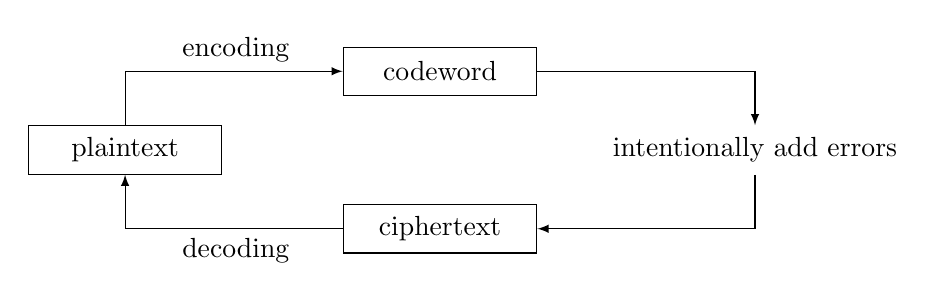
\begin{tikzpicture}
    \node[draw, minimum width=70pt, minimum height=17.5pt] (plain1) at (0, -1) {plaintext};
    \node[draw, minimum width=70pt, minimum height=17.5pt] (ciphertext) at (4, -2) {ciphertext};
    \node[draw, minimum width=70pt, minimum height=17.5pt] (codeword) at (4, 0) {codeword};
    \node[minimum width=70pt, minimum height=17.5pt] (adderror) at (8, -1) {intentionally add errors};
    \draw[-latex] (plain1) |- node[above, xshift=40pt]{encoding} (codeword);
    \draw[-latex] (codeword) -| (adderror);
    \draw[-latex] (adderror) |- (ciphertext);
    \draw[-latex] (ciphertext) -| node[below, xshift=40pt]{decoding} (plain1);
    \end{tikzpicture}
    \label{fig:code-idea}
    \fonte{the author.}
    \caption{Code-based cryptography main idea.}
\end{figure}

Based on two well know problems, the security of McEliece has remained stable. The first assumption was the hardness of generic decoding, and it is NP-complete and is also consider hard on average. The second assumption that regards the security of the McEliece scheme was the indistinguishability of the code. This second assumption is not as old as the first one, but it relates to old problems of algebraic coding theory and its consider valid for Goppa Codes, as the original proposal. 

The original parameters were designed for $2^{64}$ security bits, but it easily scales up to provide an ample security margin against attackers. Furthermore, the McEliece Cryptosystem suffers many structural attacks, and until today the original proposal is considered secure. It is important to note that many of these attacks based on the same strategy, the information set-decoding. This kind of attack does not affect schemes based on Goppa codes. However, many other families of codes suffer several drawbacks with this attack. 


As proposed in \cite{bernstein2017classic, bardet2017big} on the NIST standardization process, the McEliece cryptosystem, using binary Goppa codes, could be applied to concept a KEM, as defined in Chapter \ref{ch:math}. Based on this fact, we can generalize the cryptosystem in three algorithms: the Key generation and Encryption are defined in Section \ref{sub:mc-def} and Decryption in Section \ref{sub:mc-dec}.

\subsection{Definitions}
\label{sub:mc-def}
In this Section we describe the three main algorithms of the McEliece the McEliece cryptosystem based on irreducible binary Goppa code. 

Algorithm~\ref{alg:keygen} is the key generation of McEliece. First, it starts by generating a binary irreducible Goppa polynomial $g(z)$ of degree $t$. This random selection was made by generating a random polynomial and testing if we generated a irreducible polynomial or not.  Second, it generates the support $L$ as an ordered subset of $\mathbb{F}_{2^m}$ satisfying the root condition. Third, it is the computation of the systematic form of $\hat{H}$ is done using the Gauss-Jordan elimination algorithm. Steps four, five, and six compute the generator matrix from the previous systematic matrix and return secret and public key.


%%%%%%%%%%%%%%%%%%%%%%%%%%%%%%%%%%%%%%%%%
%%%%%%%%%%%% McEliece Key gen %%%%%%%%%%%
%%%%%%%%%%%%%%%%%%%%%%%%%%%%%%%%%%%%%%%%%
\begin{figure}
\centering
\begin{algorithm}[H]
 \KwData{$t, k, n, m$ as integers.}
 \KwResult{pk as public key, sk as secret key.}
 Select a random binary Goppa polynomial $g(z)$ of degree $t$ over $\mathbb{F}_{2^{m}}$\;
 Randomly choose $n$ distinct elements of $\mathbb{F}_{2^m}$ that are not roots of $g(z)$ as the support $L$\;
 Compute the $k \times n$ parity check matrix $\hat{H}$ according to $L$ and $g(z)$\;
 Bring $H$ to systematic form: $H_{sys} = [I_{k-n}|H']$\;
 Compute generator matrix $G$ from $H_{sys}$\;
 \Return $\quad sk = (L, g(z)) \quad pk = (G)$\;
 \caption{McEliece key generation.}
 \label{alg:keygen}
\end{algorithm}
\end{figure}

Given a public key, generated by the Algorithm \ref{alg:keygen} and a message $m$, Algorithm~\ref{alg:2} shows the encryption process of McEliece. The process is simple and efficient, requiring only a random vector $e$ with $w_h(e) \leq t$ and a multiplication of a vector by a matrix.

\begin{figure}
\centering
\begin{algorithm}[H]
 \KwData{Public key $pk = G $, message $m \in \mathbb{F}^{k}_{2}$.}
 \KwResult{$c$ as ciphertext of length $n$.}
Choose randomly an error vector $e$ of length $n$ with $w_h(e)\leq t$\;
Compute $c = (m\cdot G) \oplus e$\;
\Return $c$\;
\caption{McEliece encryption.}\label{alg:2}
\end{algorithm}
\end{figure}

\subsection{Decryption}
\label{sub:mc-dec}
Algorithm~\ref{alg:3} gives the decryption part of McEliece. This algorithm consists of the removal of the applied errors using a decoding algorithm. First, we compute the syndrome polynomial $S_c(z)$. Second, we recover the error vector $e$ from the syndrome polynomial. Finally, we can recover the plaintext $m$ computing $c \oplus e$, i.e., the exclusive-or of the ciphertext and the error vector. Note that in modern KEM versions of McEliece, $m\in \mathbb{F}^n_{2}$ is a random bit string used to compute a session key using a hash function. Hence, there is no intelligible information in seeing the first $k$ positions of $m$ with almost no error.

\begin{figure}
    \centering
    \begin{algorithm}[H]
     \KwData{$c$ as ciphertext of length $n$, secret key $sk= (L, g(z))$.}
     \KwResult{Message $m$}
     Compute the syndrome $S_c(z) = \sum{\frac{c_i}{z+\alpha_i}} \mod g(z)$\;
     Compute $\tau(z) = \sqrt{S^{-1}_{c}(z)+z}$\;
     Compute $b(z)$ and $a(z)$, so that $b(z)\tau(z) = a(z) \mod g(z)$, such that deg($a$)$\leq \lfloor \frac{t}{2} \rfloor$ and deg($b$)$\leq \lfloor \frac{t-1}{2} \rfloor$\;
     Compute the error locator polynomial $\sigma(z) = a^2(z) + zb^2(z)$ and deg($\sigma$) $\leq t$\;
     The position in $L$ of the roots of $\sigma(z)$ define the error vector $e$\;
     Compute the plaintext $m = c \oplus e$\;
     \Return $m$\;
     \caption{McEliece decryption.}\label{alg:3}
    \end{algorithm}
\end{figure}


In the decryption algorithm, steps $2$-$5$ are the description of Patterson's algorithm~\cite{patterson1975algebraic}. This same strategy can be used in schemes that make use of the Niederreiter cryptosystem~\cite{niederreiter}. As shortly described in Chapter \ref{ch:math}, these schemes differ in their public-key structure, encryption, and decryption step, but both of them, in the decryption steps, decode the message from the syndrome. Others decoding algorithm could be applied to decoding an message with error, but the main focus of this works relies on the Patterson's algorithm because of they are the most used on literature. 

The roots of the ELP can be acquired with different methods. Although these methods can be implemented with different forms, it is essential that the implementations do not leak any timing information about their execution. This leakage can lead to a side-channel attack using time differences in the decryption algorithm, as we explore in a scheme in Section~\ref{sec:attack}.

\section{BIGQUAKE}
In this Section we will describe the BIGQUAKE submission, the usage of the McEliece in their protocol and after that, we present an timing side-channel attack against the decapsulation process. The attack was original proposal in \cite{shoufan2009timing}, we use the fact that BIGQUAKE claim to be IND-CAA to create our attack scenario and perform the attack proposal.

\label{sec:attack}
\subsection{Submission overview}
BIGQUAKE~\cite{bardet2017big} uses binary Quasi-cyclic (QC) Goppa codes in order to accomplish a KEM between two distinct parts. Instead of using binary Goppa codes, BIGQUAKE uses QC Goppa codes, which have the same properties as Goppa codes but allow smaller keys.

Let us suppose that Alice and Bob ($A$ and $B$ respectively) want to share a session secret key $K$ using BIGQUAKE. Then Bob needs to publishes his public key and Alice needs to follow the encapsulation mechanism. $\mathcal{F}$ is a function that maps an arbitrary binary string as input and returns a word of weight $t$, i.e $\mathcal{F}: \{0,1\}^* \to \{x \in \mathbb{F}^n_2 | w_h(x) = t\}$. The detailed construction of the function $\mathcal{F}$ can be found at subsection $3.4.4$ in \cite{bardet2017big}. $\mathcal{H} : \{0,1\}^k \to \{0,1\}^s$ is a hash function. The function $\mathcal{H}$ in the original implementation is SHA-3. The encapsulation mechanism are describe in Protocol~\ref{prot_bigquake}.


\begin{figure}
\centering
\begin{protocol}{BIGQUAKE Key Encapsulation Mechanism between Alice and Bob}
    \label{prot_bigquake}
    \textit{Inputs.} Bob public key as a generator matrix $G$
    \sbline
    \textit{Goal.} Parties jointly agree the same session key $K$
    \sbline
    \textit{The protocol:}
    \begin{enumerate}
      \item \textbf{Encapsulation.}
      \begin{enumerate}[label=(\alph*)]
        \item Alice generates a random $m \in \mathbb{F}^s_2$;
    
        \item Generate $e \gets \mathcal{F}(m)$;
        
        \item $A$ sends $c \gets (m\oplus\mathcal{H}(e), H\cdot e^T, \mathcal{H}(m))$ to $B$;
        
        \item The session key is defined as: $K\gets \mathcal{H}(m,c)$.
      \end{enumerate}
      \item \textbf{Decapsulation.}
      \begin{enumerate}[label=(\alph*)]
        \item $B$ receives $c = (c_1,c_2,c_3)$;
        \item Using the secret key, Bob decodes $c_2$ to $e'$ with $w_h(e') \leq t$ such that $c_2 = H\cdot e'^T$;
        \item $B$ computes $m' \gets c_1\oplus\mathcal{H}(e')$;
        \item $B$ computes $e'' \gets \mathcal{F}(m')$;
        \item If $e'' \neq e'$ or $\mathcal{H}(m') \neq c_3$ then $B$ aborts.
        \item Else, $B$ computes the session key: $K\gets \mathcal{H}(m',c)$.
      \end{enumerate}
    \end{enumerate}
    \\
    \hline
\end{protocol}
\end{figure}

After Bob executes the decapsulation process successfully, both parties of the protocol agree on the same session secret key $K$. The core of the protocol are the steps which involves the McEliece encryption and decryption steps. the implementations needs to blind time variances 



\subsection{Timing side-channel attack}
In \cite{shoufan2009timing}, the attack exploits the fact that flipping a bit of the error $e$ changes the Hamming weight $w$ and per consequence the timing for its decryption. If we flip a position that contains an error ($e_i = 1$) then the error will be removed and the time of computation will be shorter. However, if we flip a bit in a wrong position ($e_i = 0$) then it will add another error, and it will increase the decryption time. The attack described in~\cite{bucerzan2017improved} exploits the root finding in the polynomial ELP. It takes advantage of sending ciphertexts with fewer errors than expected, which generate an ELP with degree less than $t$, resulting in less time for finding roots. We explore both ideas applied to the implementation of BIGQUAKE.

Algorithm~\ref{alg:attack:1} is the direct implementation of the attack proposed in~\cite{shoufan2009timing}. We reused the attack presented to show that the attack still works in current implementations such as BIGQUAKE when the root finding procedure is vulnerable to remote timing attacks. 

\begin{figure}
\centering
\begin{algorithm}[H]
 \KwData{$n$-bit ciphertext $c$, $t$ as the number of errors and precision parameter $M$}
 \KwResult{Attempt to obtain an error vector $e$ hidden in $c$.}
 $e \gets [0,\ldots,0]$\;
\For{$i\gets0$ \KwTo $n-1$}{
    $A \gets 0$\;
    $c' \gets c \oplus \text{setBit}(n,i)$\;
    $time_m \gets 0$\;
    \For{$j\gets0$ \KwTo $M$}{
        $time_s \gets time()$\;
        decrypt($c'$)\;
        $time_e \gets time()$\;
        $time_m \gets time_m + (time_e - time_s)$\;
    }
    $A \gets time_m / M$\;
    $T \gets (A, i)$\;
}
Sort $T$ in descending order of $A$\;
\For{$k\gets0$ \KwTo $t-1$}{
    $index \gets T[k].i$\;
    $e[index] \gets 1$\;
}
\Return $e$\;
 \caption{Attack on ELP.}
  \label{alg:attack:1}
\end{algorithm}
\end{figure}

After finding the position of the errors, one needs to verify if the error $e'$ found is the correct one, and then recover the message $m$. In order to verify for correctness, one can check $e'$ by computing $\mathcal{H}(e) \oplus \mathcal{H}(e') \oplus m = m'$ and if $c_3$ is equal to $\mathcal{H}(m')$. As mentioned early in this Section, the ciphertext is composed by $c = (m\oplus\mathcal{H}(e), H\cdot e^T, \mathcal{H}(m))$ or $c = (c_1, c_2, c_3)$.

\chapter{Root finding techniques and countermeasures}
\label{ch:roots}
As argued, the leading cause of information leakage in the decoding algorithm is the process of finding the roots of the ELP. In general, the time needed to find these roots varies, often depending on the roots themselves. Thus, an attacker who has access to the decoding time can infer these roots, and hence get the vector of errors $e$. Next, we propose modifications in four of these algorithms to avoid the attack presented in Subsection~\ref{sec:attack}.

Strenzke~\cite{strenzke2012fast} presents an algorithm analysis for fast and secure root finding for code-based cryptosystems. He uses as a basis for his results the implementation of ``Hymes '' \cite{hymes}. Some of that implementation uses, for instance, log and antilog tables for some operations in finite fields, which are known to be vulnerable. Given that, we rewrote those operations without tables and analyzed each line of code from the original implementations, taking care of modifying them in order to eliminate processing that could indicate root-dependent execution time. The adjustments were made in the following algorithms to find roots: exhaustive search, linearized polynomials, Berlekamp trace algorithm (BTA), and successive resultant algorithm (SRA).

One more here

\section{Exhaustive search}
The exhaustive search is a direct method, in which the evaluation of $f$ for all the elements in $\mathbb{F}_{2^m}$ is performed. A root is found whenever the evaluation result is zero. This method is acceptable for small fields and can be made efficient with a parallel implementation. Algorithm~\ref{alg:exhaustive} describes this method.

As can be seen in Algorithm~\ref{alg:exhaustive}, this method leaks information. This is because whenever a root is found, i.e., $dummy = 0$, an extra operation is performed. In this way, the attacker can infer from this additional time that a root was found, thus providing ways to obtain data that should be secret.

\begin{figure}[ht]
\begin{algorithm}[H]
 \KwData{$p(x)$ as univariate polynomial over $\mathbb{F}_{2^m}$ with $d$ roots, $A = [a_0, \ldots, a_{n-1}]$ as all elements in $\mathbb{F}_{2^m}$, $n$ as the length of $A$.}
 \KwResult{$R$ as a set of roots of $p(x)$.}
 $R \gets \emptyset$\;
\For{$i\gets0$ \KwTo $n-1$}{
    $dummy \gets p(A[i])$\;
   \If{$dummy == 0$}{
        $R.add(A[i])$\;
    }
}
\Return $R$\;
  \caption{Exhaustive search algorithm for finding roots of a univariate polynomial over $\mathbb{F}_{2^m}$.}\label{alg:exhaustive}
\end{algorithm}
\end{figure}

One solution to avoid this leakage is to permute the elements of vector $A$. Using this technique, an attacker can identify the extra operation, but without learning any secret information. In our case, we use the Fisher-Yates shuffle~\cite{black2005fisher} for shuffling the elements of vector $A$. In~\cite{wang2018fpga}, the authors show an implementation of the shuffling algorithm safe against timing attacks. Algorithm~\ref{alg:exhaustive_permuted} shows the permutation of the elements and the computation of the roots.

\begin{figure}[ht]
\begin{algorithm}[H]
 \KwData{$p(x)$ as a univariate polynomial over $\mathbb{F}_{2^m}$ with $d$ roots, $A = [a_0, \ldots, a_{n-1}]$ as all elements in $\mathbb{F}_{2^m}$, $n$ as the length of $A$.}
 \KwResult{$R$ as a set of roots of $p(x)$.}
  permute$(A)$\;
 $R \gets \emptyset$\;
\For{$i\gets0$ \KwTo $n-1$}{
    $dummy \gets p(A[i])$\;
   \If{$dummy == 0$}{
        $R.add(A[i])$\;
    }
}
\Return $R$\;
 \caption{Exhaustive search algorithm with a countermeasure for finding roots of an univariate polynomial over $\mathbb{F}_{2^m}$.}
  \label{alg:exhaustive_permuted}
\end{algorithm}
\end{figure}

Using this approach, we add one extra step to the algorithm. However, this permutation blurs the sensitive information of the algorithm, making the usage of Algorithm~\ref{alg:exhaustive_permuted} slightly harder for the attacker to acquire timing leakage.


\section{Berlekamp Trace Algorithm}
In~\cite{berlekamp1970factoring}, Berlekamp presents an efficient algorithm to factor a polynomial, which can be used to find its roots. We call this algorithm \emph{Berlekamp trace algorithm} since it works with a trace function defined as $Tr(x) = x + x^{2} + x^{2^{2}} + \dots + x^{2^{m-1}}$. It is possible to change BTA for finding roots of a polynomial $p(x)$ using $\beta = \{\beta_1, \beta_2, \ldots, \beta_m\}$ as a standard basis of $\mathbb{F}_{2^{m}}$, and then computing the greatest common divisor between $p(x)$ and $Tr(\beta_0 \cdot x)$. After that, it starts a recursion where BTA performs two recursive calls; one with the result of gcd algorithm and the other with the remainder of the division $p(x) / \gcd(p(x), Tr(\beta_i \cdot x))$. The base case is when the degree of the input polynomial is smaller than one. In this case, BTA returns the root, by getting the independent term of the polynomial. In summary, the BTA is a divide and conquer like algorithm since it splits the task of computing the roots of a polynomial $p(x)$ into the roots of two smalls polynomials. The description of BTA algorithm is presented in Algorithm~\ref{alg:bta}.

\begin{figure}[ht]
\begin{algorithm}[H]
 \KwData{$p(x)$ as a univariate polynomial over $\mathbb{F}_{2^m}$ and i.}
 \KwResult{The set of roots of $p(x)$.}
    \If{$deg(p(x)) \leq 1$}{
        \Return root of $p(x)$\;
    }
    $p_{0}(x) \gets gcd(p(x), Tr(\beta_{i}\cdot x))$\;
    $p_{1}(x) \gets p(x) / p_{0}(x)$ \;
\Return $BTA(p_{0}(x), i + 1) \cup BTA(p_{1}(x), i + 1)$\;
 \caption{Berlekamp Trace Algorithm -- $BTA(p(x), i)-rf$.}
  \label{alg:bta}
\end{algorithm}
\end{figure}

As we can see, a direct implementation of Algorithm~\ref{alg:bta} has no constant execution time. The recursive behavior may leak information about the characteristics of roots in a side-channel attack. Additionally, in our experiments, we noted that the behavior of the gcd with the trace function may result in a polynomial with the same degree. Therefore, BTA will divide this input polynomial in a future call with a different basis. Consequently, there is no guarantee of a constant number of executions. 

In order to avoid the nonconstant number of executions, here referred as $BTA-it$, we propose an iterative implementation of Algorithm~\ref{alg:bta}. In this way, our proposal iterates in a fixed number of iterations instead of calling itself until the base case. The main idea is not changed; we still divide the task of computing the roots of a polynomial $p(x)$ into two smaller instances. However, we change the approach of the division of the polynomial. Since we want to compute the same number of operations independent of the degree of the polynomial, we perform the gcd with a trace function for all basis in $\beta$, and choose a division that results in two new polynomials with approximate degree.

This new approach allows us to define a fixed number of iterations for our version of BTA. Since we always divide into two small instances, we need $t-1$ iterations to split a polynomial of degree $t$ in $t$ polynomials of degree $1$. Algorithm~\ref{alg:ibta} presents this approach.


\begin{algorithm}[ht]
 \KwData{$p(x)$ as an univariate polynomial over $\mathbb{F}_{2^m}$, $t$ as number of expected roots.}
 \KwResult{The set of roots of $p(x)$.}
    $g \gets \{p(x)\};$ \tcp{The set of polynomials to be computed}
    \For{$k \gets 0$ \KwTo $t$}{
        $current = g.pop()$\;
        Compute $candidates$ $=$ $gcd(current, Tr(\beta_{i}\cdot x))$ $\forall$ $\beta_{i}$ $\in$ $\beta$\;
        Select $p_{0}$ $\in$ $candidates$ such as $p_{0}.degree$ $\simeq$ $\frac{current}{2}$\;
        $p_{1}(x) \gets current / p_{0}(x)$ \;
        \If{$p_{0}.degree == 1$}{
            $R.add($root of $p_{0})$
        } \Else{
            $g.add(p_{0})$\;
        }
        \If{$p_{1}.degree == 1$}{
            $R.add($root of $p_{1})$
        } \Else{
            $g.add(p_{1})$\;
        }
    }
    \Return{$R\;$}
 \caption{Iterative Berlekamp Trace Algorithm -- $BTA(p(x))-it$.}
  \label{alg:ibta}
\end{algorithm}

Algorithm~\ref{alg:ibta} extracts a root of the polynomial when the variable $current$ has a polynomial with degree equal to one. If this degree is greater than one, then the algorithm needs to continue dividing the polynomial until it finds a root. The algorithm does that by adding the polynomial in a stack and reusing this polynomial in a division. 

\section{Linearized Polynomials}
The second countermeasure proposed is based on linearized polynomials. The authors in \cite{fedorenko2002finding} propose a method to compute the roots of a polynomial over $\mathbb{F}_{2^m}$, using a particular class of polynomials, called linearized polynomials. In \cite{strenzke2012fast}, this approach is a recursive algorithm which the author calls ``dcmp-rf''. In our solution, however, we present an iterative algorithm. We define linearized polynomials as follows:

\begin{definition}
A polynomial $\ell(y)$ over $\mathbb{F}_{2^m}$ is called a linearized polynomial if
\begin{equation}
    \ell(y) = \sum_i c_iy^{2^i},
\end{equation}
where $c_i \in \mathbb{F}_{2^m}$.
\end{definition}
In addition, from~\cite{truong2001fast}, we have Lemma~\ref{lemma:lin} that describes the main property of linearized polynomials for finding roots.
\begin{lemma}
\label{lemma:lin}
    Let $y \in \mathbb{F}_{2^m}$ and let $\alpha^0, \alpha^1, \ldots, \alpha^{m-1}$ be a standard basis over $\mathbb{F}_2$. If
    \begin{equation}
        y = \sum_{k=0}^{m-1} y_k\alpha^k, y_k \in \mathbb{F}_2
    \end{equation}
    and $\ell(y) =\sum_j c_jy^{2^j}$, then
      \begin{equation}
        \ell(y) = \sum_{k=0}^{m-1} y_k\ell(\alpha^k).
    \end{equation}
\end{lemma}

We call $A(y)$ over $\mathbb{F}_{2^m}$ as an affine polynomial if $A(y) = \ell(y) + \beta$ for $\beta \in \mathbb{F}_{2^m}$, where $\ell(y)$ is a linearized polynomial.

We can illustrate a toy example to understand the idea behind finding roots using linearized polynomials.
\begin{example}\label{ex:1}
Let us consider the polynomial $f(y) = y^2 + (\alpha^2+1)y + (\alpha^2 +\alpha +1)y^0$ over $\mathbb{F}_{2^3}$ and $\alpha$ are elements in $\mathbb{F}_2[x]/ x^3+x^2+1$. Since we are trying to find roots, we can write $f(y)$ as
 $$ y^2 + (\alpha^2+1)y + (\alpha^2 +\alpha +1)y^0 = 0$$
 or
\begin{equation}\label{eq:example_1}
    y^2 + (\alpha^2+1)y   = (\alpha^2 +\alpha +1)y^0
\end{equation}
We can point that on the left hand side of Equation~\ref{eq:example_1}, $\ell(y) = y^2 + (\alpha^2+1)y$ is a linearized polynomial over $\mathbb{F}_{2^3}$ and Equation~\ref{eq:example_1} can be expressed just as
\begin{equation}\label{eq:example_1_2}
    \ell(y) = \alpha^2 +\alpha +1
\end{equation}
If $y = y_2\alpha^2 + y_1\alpha + y_0 \in \mathbb{F}_{2^3}$ then, according to Lemma~\ref{lemma:lin}, Equation~\ref{eq:example_1_2} becomes
\begin{equation}\label{eq:example_1_3}
    y_2\ell(\alpha^2) + y_1\ell(\alpha) + y_0\ell(\alpha^0) = \alpha^2 +\alpha +1
\end{equation}
We can compute $\ell(\alpha^0),\ell(\alpha)$ and $\ell(\alpha^2)$ using the left hand side of Equation~\ref{eq:example_1} and we have the following values
\begin{equation}\label{eq:example_1_4}
    \begin{split}
        \ell(\alpha^0) & = (\alpha^0)^2 + (\alpha^2+1)(\alpha^0) = \alpha^2+1 + 1 = \alpha^2 \\
        \ell(\alpha) & = (\alpha)^2 + (\alpha^2+1)(\alpha) = \alpha^2 + \alpha^2+ \alpha + 1 = \alpha + 1 \\
        \ell(\alpha^2) & = (\alpha^2)^2 + (\alpha^2+1)(\alpha^2) = \alpha^4 +\alpha^4 +  \alpha^2 = \alpha^2.
    \end{split}
\end{equation}
A substitution of Equation~\ref{eq:example_1_4} into Equation~\ref{eq:example_1_3} gives us
\begin{equation}\label{eq:example_1_5}
     (y_2+y_0)\alpha^2 + (y_1)\alpha + (y_1)\alpha^0 = \alpha^2 +\alpha +1
\end{equation}
Equation~\ref{eq:example_1_5} can be expressed as a matrix in the form
\begin{equation}\label{eq:example_1_6}
    \begin{bmatrix} y_2 & y_1 & y_0 \end{bmatrix}
    \begin{bmatrix}
    1 & 0 & 0 \\
    0 & 1 & 1 \\
    1 & 0 & 0
    \end{bmatrix}
    =
    \begin{bmatrix} 1 & 1 & 1 \end{bmatrix}.
\end{equation}
If one solves simultaneously the linear system in Equation~\ref{eq:example_1_6} then the results are the roots of the polynomial given in Equation~\ref{eq:example_1}. From Equation~\ref{eq:example_1_5}, one observes that the solutions are $y=110$ and $y=011$, which can be translated to $\alpha + 1$ and $\alpha^2 + \alpha$.
\end{example}


Fortunately, the authors in \cite{fedorenko2002finding} provide a generic decomposition for finding affine polynomials. In their work, each polynomial in the form $F(y) = \sum_{j=0}^{t} f_jy^j$ for $f_j \in \mathbb{F}_{2^m}$ can be represented as
\begin{equation}
\label{eq:f_y}
    F(y) = f_3y^3 + \sum_{i=0}^{\lceil (t-4)/5 \rceil} y^{5i}(f_{5i} + \sum_{j=0}^{3} f_{5i+2^j}y^{2^j})
\end{equation}
After that, we can summarize all the steps as Algorithm~\ref{alg:linearized}. The function ``generate($m$)'' refers to the generation of the elements in $\mathbb{F}_{2^m}$ using Gray codes, see \cite{savage1997survey} for more details about Gray codes. Algorithm~\ref{alg:linearized} presents a countermeasure in the last steps of the algorithm, i.e., we added a dummy operation for blinding if $X[j]$ is a root of polynomial $F(x)$.

\begin{figure}
\begin{algorithm}[H]
 \KwData{$F(x)$ as a univariate polynomial over $\mathbb{F}_{2^m}$ with degree $t$ and $m$ as the extension field degree.}
 \KwResult{$R$ as a set of roots of $p(x)$.}
 $\ell^k_i \gets \emptyset$; $\ell_{is} \gets \emptyset$; $A^j_k \gets \emptyset$; $R \gets \emptyset$; $dummy \gets \emptyset$\;
 \If{$f_0  == 0$}{
 $R.append(0)$\;
 }
 \For{$i\leftarrow 0$ \KwTo $\lceil (t-4)/5 \rceil$}
 {
    $\ell_i(x) \gets 0$\;
    \For{$j\gets 0$ \KwTo $3$}{
      $\ell_i(x) \gets \ell_i(x) + f_{5i+2^j}x^{2^j}$\;
      }
    $\ell_{is}[i] \gets \ell_i(x)$\;
 }
 \For{$k\gets 0$ \KwTo $m-1$}{
    \For{$i\leftarrow 0$ \KwTo $\lceil (t-4)/5 \rceil$}
    {
        $\ell^k_i \gets \ell_{is}(\alpha^k)$\;
    }

 }
 $A^0_i \gets \emptyset$\;
 \For{$i\gets 0$ \KwTo $\lceil (t-4)/5 \rceil$}{
  $A^0_i \gets f_{5i}$\;
 }

 $X \gets \text{generate}(m)$\;
 \For{$j\gets 1$ \KwTo $2^m - 1$}{
    \For{$i\gets 0$ \KwTo $\lceil (t-4)/5 \rceil$}{
        $A \gets A^{j-1}_i$\;
        $A \gets A + \ell^{\delta(X[j], X[j-1])}_i$\;
        $A^j_i \gets A$\;
    }
 }
\For{$j\gets 1$ \KwTo $2^m - 1$}{
    $result \gets 0$\;
    \For{$i\gets 0$ \KwTo $\lceil (t-4)/5 \rceil$}{
        $result = result + (X[j])^{5i}A^j_i$\;
    }
    $eval = result + f_3(X[j])^{3}$\;
    \eIf{$eval == 0$}{
        $R.append(X[j])$\;
    }{
        $dummy.append(X[j])$\;
    }
}
\Return $R$\;
 \caption{Linearized polynomials for finding roots over $\mathbb{F}_{2^m}$.}
  \label{alg:linearized}
\end{algorithm}
\end{figure}

\section{Successive Resultant Algorithm}
In \cite{petit2014finding}, the authors present an alternative method for finding roots in $\mathbb{F}_{p^m}$. Later on, the authors better explain the method in~\cite{petit2016finding}. The Successive Resultant Algorithm (SRA) relies on the fact that it is possible to find roots exploiting properties of an ordered set of rational mappings.

Given a polynomial $f$ of degree $d$ and a sequence of rational maps $K_1,\ldots, K_t$, the algorithm computes finite sequences of length $j \leq t+1$ obtained by successively transforming the roots of $f$ by applying the rational maps. The algorithm is as follows: Let $\{v_1,\ldots,v_m\}$ be an arbitrary basis of $\mathbb{F}_{p^m}$ over $\mathbb{F}_p$, then it is possible to define $m+1$ functions $\ell_0, \ell_1,\ldots, \ell_m$ from $\mathbb{F}_{p^m}$ to $\mathbb{F}_{p^m}$ such that
$$
\left \{
\begin{array}{l}
     \ell_0(z) = z\\
     \ell_1(z) = \prod_{i\in \mathbb{F}_p}\ell_0(z-iv_1)\\
     \ell_2(z) = \prod_{i\in \mathbb{F}_p}\ell_1(z-iv_2)\\
     \cdots \\
     \ell_m(z) = \prod_{i\in \mathbb{F}_p}\ell_{m-1}(z-iv_m)\\
\end{array}
\right.
$$
The functions $\ell_j$ are examples of linearized polynomials, as previously defined in Chapter~\ref{ch:math}. Our next step is to present the theorems from \cite{petit2014finding}. Check original work for the proofs.
\begin{theorem}\label{lemma_1}
\begin{itemize}
    \item[a)] Each polynomial $\ell_i$ is split and its roots are all elements of the vector space generated by $\{v_1, \ldots,v_i\}$. In particular, we have $\ell_n(z) = z^{p^m} -z$.
    \item[b)] We have $\ell_i(z)  = \ell_{i-1}(z)^p - a_i\ell_{i-1}(z)$ where $a := (\ell_{i-1}(v_i))^{p-1}$.
    \item[c)] If we identify $\mathbb{F}_{p^m}$ with the vector space $(\mathbb{F}_p)^m$, then each $\ell_i$ is a $p$-to-$1$ linear map of $\ell_{i-1}(z)$ and a $p^i$ to $1$ linear map of $z$.
\end{itemize}
\end{theorem}

From Theorem~\ref{lemma_1} and its properties, we can reach the following polynomial system:
\begin{equation}\label{eq:system_1}
    \left \{
\begin{array}{l}
    f(x_1) = 0\\
     x_j^p = a_jx_j = x_{j+1} \quad j=1,\ldots, m-1\\
     x_n^p - a_nx_n = 0
\end{array}
\right.
\end{equation}
where the $a_i \in \mathbb{F}_{p^n}$ are defined as in Theorem~\ref{lemma_1}. Any solution of this system provides us with a root of $f$ by the first equation, and the $n$ last equations together imply this root belongs to $\mathbb{F}_{p^n}$. From this system of equations,~\cite{petit2014finding} derives Theorem~\ref{lemma_2}.

\begin{theorem}\label{lemma_2}
Let $(x_1,x_2,\ldots,x_m)$ be a solution of the equations in Equation~\ref{eq:system_1}. Then $x_1 \in \mathbb{F}_{p^m}$ is a solution of $f$. Conversely, given a solution $x_1 \in \mathbb{F}_{p^m}$ of $f$, we can reconstruct a solution of all equations in Equation~\ref{eq:system_1} by setting $x_2 =x_1^p - a_1x_1$, etc.
\end{theorem}

In \cite{petit2014finding}, the authors present an algorithm for solving the system in Equation~\ref{eq:system_1} using resultants. The solutions of the system are the roots of polynomial $f(x)$. It is worth remarking that this algorithm is almost constant-time and hence we just need to protect the branches presented on it.


\section{Cantor-Zassenhaus Algorithm}


\chapter{Comparison}
\label{ch:comparison}
In this chapter we will present an analysis over the five presented method on previous section. The first two analysis has focus on the complexity and performance of the algorithms. However, we are not interested only in efficient methods, our main goal was achieve an method with no information leakage against a timing side-channel attack. Hence, we demonstrate an time-variance analysis for each proposed root-finding method. After that, we present an security analysis over the algorithm. Remarking that, $m$ are the extension, $n = 2^m$, and $t$ the degree of polynomial.

\section{Complexity analysis}
In order to compare the complexity of the algorithm, we use the Big $\mathcal{O}$ notation. This asymptotic notation permits to us classify the algorithms according to their behaviour when the inputs grows. 




\begin{table}[ht]
\centering
\label{tab:complexity}
\caption{Complexity comparison}
\begin{tabular}{ll}
Method                                  &                \\ \hline
Exhaustive search                       & $\mathcal{O}(2^mt)$ \\
Permuted exhaustive                     & $\mathcal{O}(2^mt)$ \\
Linearized Polynomials                  & $\mathcal{O}(2^m)$ \\
Constant Linearized Polynomials         & $\mathcal{O}(2^m)$ \\
Berlekamp trace algorithm               & $\mathcal{O}(mt^2)$ \\
Iterative Berlekamp trace algorithm     & $\mathcal{O}(mt^2)$ \\
Successive resultant algorithm          & $\mathcal{O}(t^2m^3)$ \\
Constant Successive resultant algorithm & $\mathcal{O}(t^2m^3)$ \\
Rabin root finding                      & $\mathcal{O}(t^2 \log{n})$
\end{tabular}
\end{table}

As we can note, the most asymptotic efficient method was the Rabin root finding method. However, this asymptotic could not reflect the execution timing of the algorithm for parameters used in code-based schemes. This happens because the big $\mathcal{O}$ notation does not consider constants and the asymptotic complexity was for all $m$ and $t$ grater then $m_0$ and $t_0$, and the parameters used on code-based cryptosystems could be smaller then the $m_0$ and $t_0$. To present a more 

\section{Performance analysis}
\section{Time variance analysis}
\section{Security analysis}

\chapter{Final Considerations}
\label{ch:final}
In this thesis we propose countermeasures to be applied on root finding algorithms in order to achieve a decoding process without leak any sensitive information against a timing side-channel attack. We propose five methods, with different characteristics which can be applied to the root extraction task. Our proposals are based on reduce the time variance, by applying implementation techniques which aims to construct a algorithm without branches and with a constant behaviour. 

Before present the countermeasures, we present a 

\section{Future works}
For future work, we 

%%%%%%%%%%%%%%%%%%%%%%%%%%%%%%%%%%%%%%%%%%%%%%%%%%%%%%%%%%%%%%%%%%%%
%%%                   Elementos pós-textuais                     %%%
%%%%%%%%%%%%%%%%%%%%%%%%%%%%%%%%%%%%%%%%%%%%%%%%%%%%%%%%%%%%%%%%%%%%
\postextual
\bibliography{main}
\end{document}
